%! Author = Saeid Yazdani
%! Date = 11/30/2023


\section{Design and Test Integration}
\label{sec:dfx}


As manufacturing technology and methods of electronic components and
integrated circuits progressed, a multitude of testing procedures
and strategies have been developed.
Testing is under the umbrella of guidelines and
principles, which have been accumulated over the years, named \ac{DfX}.

\ac{DfX}\footnote{Also referred to as \emph{Design for eXcellence}.} is a set of
principles to design quality products in multiple industries, including
electronics industry at the chip, board and system level, and is regarded as a key
to successful product realization \autocite{Adham}.

\begin{figure}[htbp]
    \centering
    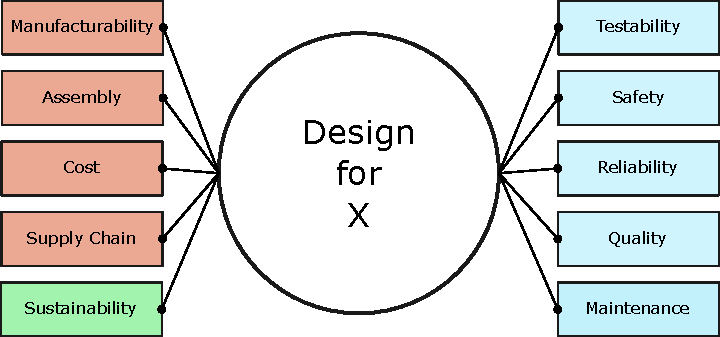
\includegraphics[width=0.86\linewidth,height=0.50\textheight,keepaspectratio]
    {figures/design-for-x}
    \caption[Design for X]{\ac{DfX} and its most important aspects.}
    \label{fig:dfx-chart}
\end{figure}

The "X" in \ac{DfX} stands for different variables (\autoref{fig:dfx-chart})
that are crucial in the product development process and can vary depending on
the particular focus or objective of the design to ensure a successful release
of a product to the market by providing guidelines in multiple domains of the
production pipeline:

\begin{itemize}[topsep=8pt,itemsep=4pt,partopsep=4pt, parsep=4pt]

    \item \textbf{\emph{\ac{DfT}:}} Ensures that a product is designed to be
    testable, facilitating the detection of defects and simplifying the test
    process.

    \item \textbf{\emph{\ac{DfM}:}} Focuses on designing products to be simple
    and cost-effective to manufacture. It involves simplifying the design,
    reducing parts, and ensuring ease of assembly.

    \item \textbf{\emph{\ac{DfA}:}} Aims to reduce the product assembly cost and
    complexity by minimizing the number of assembly operations, facilitating
    easier assembly processes, and often combining DfM principles.

    \item \textbf{\emph{\ac{DfC}:}} Approach to minimize the costs associated
    with the product throughout its lifecycle without compromising on quality.

    \item \textbf{\emph{\ac{DfQ}:}}  Involves designing for the product's
    performance and reliability to meet customer expectations and reduce the
    likelihood of failures.

    \item \textbf{\emph{\ac{DfR}:}} Ensures that the product will perform as
    expected without failure for a specified period under pre-defined
    conditions.

    \item \textbf{\emph{\ac{DfS}:}} Provides a set of standards to make sure
    that the product is safe to use and hazards are avoided to protect users and
    operators.

    \item \textbf{\emph{\ac{DfSu}:}} Regards the environmental considerations to
    minimize the environmental impact of a product through careful material
    selection, energy efficiency, and ensures the product is recyclable at the
    end-of-life.

    \item \textbf{\emph{\ac{DfMt}:}} Aims to design products so that they are
    easy to maintain and service, resulting in reduced downtime and maintenance
    costs.

\end{itemize}
